% This document provides the style to be used for a MSc Thesis at the
% Parallel and Distributed Systems group
\documentclass[11pt,twoside,a4paper,openright]{report}

% math packages
\usepackage{amsmath}
\usepackage{amssymb}
\usepackage{mathtools}
\usepackage{amsthm}

% textblocks for title page
\usepackage[absolute]{textpos}

% use babel for proper hyphenation
\usepackage[british]{babel}

% Graphics: different for pdflatex or dvi output, choose one
%%\usepackage[dvips]{graphicx}
%%\usepackage[pdftex]{graphicx}
\usepackage{graphicx}

\usepackage{epstopdf}
\usepackage{rotating}
\usepackage{subfigure}

% FONT
\usepackage[scaled=.92]{helvet}
%\usepackage{times}

% for url's use "\url{http://www.google.com/}"
\usepackage{url}
\usepackage[plainpages=false]{hyperref} 


\usepackage{enumitem}

\usepackage[colorinlistoftodos,prependcaption,textsize=tiny]{todonotes}

\usepackage{tikz}
\usetikzlibrary{positioning,arrows}

\tikzset{
  block/.style={
    draw,
    rectangle,
    minimum height=1cm,
    minimum width=1cm,
    align=center
  },
  subblock/.style={
    draw,
    rectangle,
    minimum height=.75cm,
    minimum width=1.5cm,
    align=center
  },
  line/.style={->,>=latex},
  XOR/.style={draw,circle,append after command={
        [shorten >=\pgflinewidth, shorten <=\pgflinewidth,]
        (\tikzlastnode.north) edge (\tikzlastnode.south)
        (\tikzlastnode.east) edge (\tikzlastnode.west)
        }
    }
}






% Information that will be filled in at various points in the report
\newcommand{\reportTitle}{Leveraging VLC for energy disaggregation in Smart Buildings}
\newcommand{\reportAuthor}{Johnny Verhoeff}
\newcommand{\reportEmail}{j.s.c.j.verhoeff@student.tudelft.nl}
\newcommand{\reportUrlEmail}{\href{mailto:\reportEmail}{\reportEmail}}
\newcommand{\reportMSC}{Embedded Systems} %{Embedded Systems}{Computer Engineering}{Computer Science}{Electrical Engineering}
\newcommand{\reportDate}{\today} %TODO: Dit is de datum van uitgifte van final versie aan de afstudeer commissie 
\newcommand{\presentationDate}{24th October 2016} %TODO: Dit is de datum van de afstudeerpresentatie 
\newcommand{\graduationCommittee}{

Chair: Prof. dr. K.G. Langendoen, Faculty EEMCS, TU Delft \\
Committee member: dr. ir. L.M. Ramirez Elizondo, Faculty DCE\&S, TU Delft \\ 
Committee member: dr. ir. M.A. Z\'u\~niga Zamalloa, Faculty EEMCS, TU Delft \\


} 
\newcommand{\reportAbstract}{TODO ABSTRACT}
\newcommand{\reportKeywords}{TODO KEYWORDS}

% For pdflatex
\pdfinfo{
   /Author (\reportAuthor)
   /Title  (\reportTitle)
   /Keywords (\reportKeywords)
}

\begin{document}

\pagenumbering{alph}
\pagestyle{empty}


% FRONTCOVER
\include{template/frontcover}

%%%%%%%%%%%%%%%%%%%%%%%%%%%%%%%%%%%%%%%%%%%%%%%%%%%%%%%%%%%%%%%%%%%%%%%%%%%%%%%
\hoffset=1.63cm
\oddsidemargin=0in
\evensidemargin=0in
\textwidth=5in

%%%%%%%%%%%%%%%%%%%%%%%%%%%%%%%%%%%%%%%%%%%%%%%%%%%%%%%%%%%%%%%%%%%%%%%%%%%%%%%
\parindent=1em

% EMPTY PAGE
\cleardoublepage

\pagestyle{plain}
\pagenumbering{roman}
\setcounter{page}{1}

% TITLE PAGE: page i (hidden)
\include{template/titlepage}

% GRADUATION DATA AND ABSTRACT: pages ii and iii (hidden)
\include{template/graduationdata}
%\setcounter{page}{4}

% EMPTY PAGE: page iv
\cleardoublepage

% OPTIONAL QUOTATION: page v
%\include{quotation}
% EMPTY PAGE: page vi
%\cleardoublepage

% PREFACE: page v
% !TeX root = ../thesis.tex

\chapter*{Preface}
\addcontentsline{toc}{chapter}{Preface}



This Master thesis is the final part of the Master of Science in the Embedded Systems program I followed at Delft University of Technology.
Prior to this thesis, I had little knowledge of VLC or energy disaggregation.
Using VLC in combination with energy disaggregation has not been explored yet.
The first steps towards disaggregating individual lights are taken in this thesis.
There are experimental results achieved as well as theoretical results.







\vspace{1\baselineskip}

\noindent



First, I would like to thank my loving family, who have supported me throughout this nine-month thesis project.
I would also like to thank my advisor Marco Z\'u\~niga Zamalloa and Akshay Narashiman for their guidance to help me finish my thesis.
Finally I want to acknowledge Koen Langendoen and Laura Ramirez Elizondo for being members of my graduation committee.







\vspace{1\baselineskip}

\noindent
Johnny Verhoeff

\vspace{1\baselineskip}

\noindent
Delft, The Netherlands

\noindent
\today

% EMPTY PAGE: page vi
\cleardoublepage

% TABLE OF CONTENTS: starting at page vii
\tableofcontents

\cleardoublepage

\pagenumbering{arabic}
\setcounter{page}{1}


\setlength{\parskip}{\baselineskip}%
%\setlength{\parindent}{0pt}%


% INTRODUCTION: page 1
% !TeX root = ../../thesis.tex

\chapter{Introduction}
\label{chp:introduction}

\vspace{1\baselineskip}

\noindent

%\vspace{1\baselineskip}

In a world where the vast majority of consumed energy, is provided by unsustainable fossil fuels~\cite{kolter2011redd}, the amount of energy we use must be reduced.
Reducing energy consumption requires knowing which devices are actually consuming the energy.
When consumers are given feedback about their energy consumption, energy savings can be made (up to 15 \% according to \cite{darby2006effectiveness}).
If a consumer knows which devices are actually using energy, he or she can decide if those devices really need to be used at that particular time.
If a device is on but it is not being used, the energy used to power it, is essentially wasted.
For example, lights on in a room which is not occupied.



Current energy meters give an aggregate power consumption, which cannot tell a consumer which specific device is responsible for the observed energy consumption or waste thereof.
This is where energy disaggregation comes in.
Energy disaggregation aims to break down the aggregate power consumption of, for example a household, to tell the consumer which devices consumes power at which times.




Energy disaggregation has been applied successfully to identify the operation of appliances, such as refrigerators and HVAC \cite{kolter2011redd} \cite{spiegel2014energy}.
Identifying the energy consumption of other devices such as lighting has not been so successful \cite{spiegel2014energy} \cite{batra2015neighbourhood}.
Each appliance in a household draws power in a certain way, this can be thought of as a signature of that appliance.
As can be seen from \autoref{fig:energy-consumption-house}, appliances such as the washer dryer and the dishwasher can be distinguished from the aggregated power draw.
These appliances can be recognized by their signature: the amount of time they draw power, how large the power draw is and if it has a recurring pattern.
For example, the refrigerator can be easily recognized due its periodic pattern, captured by the light blue peaks in \autoref{fig:energy-consumption-house}.
But the lighting can not be disaggregated on a per lamp basis.
The reason for this, is that most lighting fixtures do not have a unique signature, instead many lights have the same signature.
Disaggregating the energy consumed by lighting is important, because it is the third largest energy consumer in the average home \cite{batra2015neighbourhood}.
In buildings, lighting consumes around 30 \% of the total energy consumption \cite{halonen2010guidebook}.
In the EU as well as in the USA, approximately 11 \% of all the energy produced is used only for lighting \cite{bertoldi2009electricity} \cite{outlook2010energy}.

\begin{figure}[t]
	\centering
	\includegraphics[width=\textwidth]{chapters/introduction-chapters/energy-consumption-house.png}
	\caption{An example of energy consumption of a household over the course of a day \cite{kolter2011redd}.}
	\label{fig:energy-consumption-house}
\end{figure}




If every light in a household would have a unique power draw that is distinguishable from all other lights, the consumer can get better insight about how lighting is being used in his household. 
With this feedback, a consumer can see which individual lights are being used in the middle of the day for example or in an unoccupied room.
The consumer can then turn the lights off.
Thereby saving energy and monetary costs.



Without adding extra infrastructure, giving each light a unique signature is an almost intractable problem.
But the advent of smart lights can help with this.
Smart lights can use VLC (Visible Light Communication).
VLC is a short-range optical means of wireless communication using the visible light spectrum.
It modulates data by turing the light on and off at high frequencies so that no flickering effects can be seen by the human eye.
When a light is transmitting data via VLC, the current signature of the light changes.
%The unique power draw of each light can be managed through VLC .
%With this information that is being sent via VLC, the light can act as a beacon for indoor localization \cite{Kuo:2014:LIP:2639108.2639109}.
%For example a smart-phone could then locate itself inside a building with good accuracy.
%The ID of the LED beacon which is sent via VLC will also propagate via the current that the LED draws.
%The information that is transmitted using VLC, will also propagate via the current that the LED draws.
The current signature of a light can then be decoded with a smart-meter.
And in this way, real-time information of lights in the home building is acquired.







% !TeX root = ../../thesis.tex


\section{Problem Definition}

Energy disaggregation can detect energy consumers based off the distinct power draw that these devices have.
What it cannot yet do, is the disaggregation of appliances that have very similar power draw, such as lighting.


% !TeX root = ../../thesis.tex


\section{Thesis Contributions}

The aim of this thesis is to propose a framework consisting of theoretical methods, hardware and software, so that lights with similar power draw can be distinguished with a single smart-meter.
This thesis takes advantage of advances in two areas: CDMA codes and VLC.

The specific contributions of this thesis are:

\begin{itemize}

	\item Coding methods are analyzed to allow each LED to have a unique power draw. 
	These codes make it possible to identify if an LED is on or off, even when multiple LEDs are modulating and thereby interfering with each others unique current signature.




	\item Hardware is introduced to allow the LEDs to be modulated by a micro-controller. 
	This will allow the LEDs to propagate their unique signatures via either AC or DC. 
	And there is also hardware introduced that can sample the current at a high frequency via either AC or DC.
	The sampled current is then processed by another separate micro controller, which can then state which LEDs are on and which or off.




	\item An evaluation of the proposed hardware and software is carried out, with a testbed which uses standard LED light fixtures. For larger scale evaluations, software simulation is used. 
\end{itemize}


% !TeX root = ../../thesis.tex

\section{Thesis Organization}

The remainder of this thesis is organized as follows.
First related work is discussed in \autoref{chp:state-of-the-art}.
Then the design requirements are outlined in \autoref{chp:design-requirements}.
In \autoref{chp:cdma} the theory is explained.
Next, in \autoref{chp:hardware-design}, the design of the hardware is discussed.
In \autoref{chp:evaluation} the hardware and software is evaluated.
Finally the work is concluded in \autoref{chp:conclusionsandfuturework} and future work is identified.


% !TeX root = ../../thesis.tex

\chapter{State-of-the-Art}
\label{chp:state-of-the-art}

Text about smart grids.



Text about VLC.



Text about PLC, and drawbacks...

% !TeX root = ../../thesis.tex

\chapter{Design Requirements}
\label{chp:design-requirements}


In this section we introduce the main requirements for our system. The overall architecture has three main components: the codes, the modulator and the meter. 
These components were shown in \autoref{fig:overview-diagram} 
In this figure multiple lights can be seen.
We want to monitor which lights are on and off in a timely manner, by only looking at the energy signature of each LED.
To do this, three things must be investigated: How to construct the IDs, what hardware to use for the modulators and how to sample and process the current.
First, the requirements for the IDs will be discussed.
Next, the modulator is discussed. 
This piece of hardware will be responsible for the transmission of the ID via VLC.
This data can be used for applications such as indoor localization.
This hardware is also responsible for translating the ID into a current signature.
Finally, the smart-meter will be discussed.
The meter must sample the current that is drawn by all the LEDs.
And process that data into status indicators for each LED.








	\section{Encoding}

	To be able to distinguish multiple lights from each other, which are all connected in parallel, each light must have a unique identification sequence of some sort.
	Furthermore, that identification sequence must somehow be detected and interpreted by a smart-meter.


	The most common way to use VLC with LEDs, is to use on-off keying (OOK).
	OOK works by turning the LED on or off.
	If a data bit `1' needs to be transmitted, the LED is turned on.
	If a data bit `0' needs to be transmitted, the LED is turned off.
	This is how the information is transmitted.
	Since the LED is turning on and off according to the ID in an OOK fashion, this ID will also propagate in the current that this LED draws.
	This unique current signature flows through the smart meter.
	If only a single light is used with an ID, the meter can search for only that ID.
	If it finds that ID, the light is ON, else the lights is off.


	A problem rises when more than one light source is sending its identification sequence.
	Since the lights are connected in parallel, the current that flows through the smart meter will be the sum of all the currents that are drawn by all the light sources.
	This means that the light sources, which are effectively transmitters, interfere with each other.
	Because of that interference the unique identification sequences which are assigned to each light source, need to be carefully selected.


	To build the necessary codes we borrow from the field of telecommunications.
	In that field, similar issues occurred: For example multiple cellphones transmitting to the same base station, at the same time, at the same frequency. 
	The solution was to use code sequences that do not interfere with each other.
	The specific codes are called Orthogonal codes and Pseudo random noise codes.
	For our scenario, the codes need to satisfy the following requirements:
	\begin{itemize}

		\item The codes should be detectable with good accuracy:
		\begin{itemize}
			\item A code sequence must be able to be detected, even when multiple codes are aggregated.

			\item The codes must have as little interference as possible with each other, so that a large number of LEDs can transmit at the same time and still achieve accurate results when the smart-meter tries to detect which LEDs are transmitting.
		\end{itemize}


		\item The codes need to work in a synchronous and asynchronous manner. 
		The synchronous case is represented by scenarios where multiple in a single room can be all switched on together.
		But when there are multiple lights in multiple rooms they need not be turned on or off at the same time, this is the asynchronous case.

		\item The system must be scalable:
		\begin{itemize}
			\item The codes should not be too long, because the system must identify each LED as being on or off in a timely manner.
			The longer the code, the longer it takes to transmit this code.

			\item The number of codes that can be used must scale well.
			In other words: The number of codes that can be constructed, should be proportional to the length of the codes.  

		\end{itemize}

	\end{itemize}
	

	The exact properties, benefits and drawbacks of the codes and how they can be used in both DC and AC environments will be discussed in \autoref{chp:cdma}.




	\section{LED Modulator}

	A piece of hardware is needed to modulate the commercial LED.
	This hardware needs to translate the unique identification sequence that is assigned to each light source and modulate the LED.
	Contrary to standard VLC, which is only concerned with modulating the light intensity to transmit data, the same data must also be transmitted via the current draw.
	The modulator must not only turn the light on or off, but it must also make sure that the current that is drawn can be decoded later on by the smart-meter.
	The hardware should also allow for fast modulation to avoid seeing flickering effects.


	For the design of this hardware, or when using pre-designed hardware, the way the identification sequence translates to the current draw needs to be taken in mind.
	Since OOK is used, the modulator should ideally draw zero current when a `0' data bit is transmitted and draw a certain amount of constant current when a `1' data bit is to be transmitted.
	This current draw translation should be the case irrespective of using DC or AC.
	In a DC environment the modulator hardware will get a constant voltage, so there are no extra challenges.
	But in an AC environment the modulator will get an alternating voltage, which is not constant. 
	This will introduce multiple challenges, which will be discussed in \autoref{sec:ac-environment}.



	\section{Smart Meter}

	The smart meter needs to be able to detect relatively small current changes.
	More concretely, it needs to be able to detect the current change when even a single light is modulating.

	When selecting a method of measuring the current these points need to be taken into consideration:

	\begin{itemize}
		\item The speed at which the current can be sampled needs to be high enough to be able to correctly sample the current as the LEDs are modulating.

		\item The noise introduced in the samples must be low enough to detect the correct modulation of even one LED with consistency.
		%The accuracy of the samples being taken needs to be high enough, so that the modulation of one LED can be detected with consistency.
		%In other words, the noise of the samples must be low enough to detect the correct modulation of even one LED.

		\item The sensitivity of the meter must balance a tradeoff between the ability to detect an LED and the likelihood of getting saturated.
		%The sensitivity of the measuring method needs to be chosen such that an ADC of a micro-controller can measure the current.
		%The sensitivity must also not be too low. 
		%In combination with a too low resolution ADC this may cause the failure to detect the modulation of one LED.
		%But the sensitivity must also not be too high.
		%If it is too high, the ADC can be saturated, causing it to only be able to detect two LEDs modulating while the other LEDs are not detected.

	\end{itemize}




















% !TeX root = ../../thesis.tex

\chapter{Code Divison Multiple Access}
\label{chp:cdma}

\todo{Should I explain differences TDM/FDM/CDMA ??}

This chapter will explain which CDMA codes are considered and how to measure their performance.
The way in which these codes can be constructed is also explained, as is the environments in which they work well and work poorly. 

% !TeX root = ../../thesis.tex

\section{Performance Metrics of a CDMA Sequence}
\label{sec:performance-metrics-cdma}

To be able to objectively determine which code sequence is the best for certain environments, metrics are needed to compare the performance of a sequence.
Such metrics are: auto- and cross-correlation, length of the code and how many unique codes can be produced which are in the same set, meaning with the same length, so that they can be used together in the same system.
Also if the codes can be used in a synchronous only or in an a-synchronous environment has to be considered.


Correlation is a measure for determining how much sequence $X$ is similar to sequence $Y$ and can be found in \autoref{eq:correlation}.
With $L$ being the length of the code and $\tau$ the time-shift.
When sequence $X$ and $Y$ are the same sequence, we speak of the autocorrelation.
When they are two different sequences, we speak of the cross-correlation. 

\begin{equation}
	R(\tau)_{xy} = \displaystyle\sum_{i = 0} ^ {L - 1} x(i) \times y(i + \tau) {\text{  with $\tau = 0, 1, 2, \dotsc, L$}}
	\label{eq:correlation}
\end{equation}


%commented out because this will never be used and therefor only adds unnecessary text

%Another way to calculate the correlation between two sequences is to count the number of agreements and disagreements between the two sequences, see \autoref{eq:correlation-a-d}, this comes in handy when comparing two digital sequences, which both have $0$ and $1$ signal levels.

%\begin{equation}
%	R(\tau) = \text{\# of agreements} - \text{\# of disagreements} 
%	\label{eq:correlation-a-d}
%\end{equation}




The properties of an ideal set of codes should be, that the autocorrelation for each code in the set should be $0$ for each time-shift $\tau \neq 0$, at $\tau = 0$ the autocorrelation should be $L$, this value would than be a peak value for which we can identify if this code is present in the received signal.
If the signal is the sampled current and the code is the ID of a LED, then we can say the LED is on when the auto-correlation peak is seen.
The ideal cross-correlation properties should be $0$ for every time-shift $\tau$, so that no code interferes with any other code, hereby causing no MAI (Multiple Access Interference).



The length of a code is also of importance, because each chip of the code has to be transmitted.
Assuming a constant modulating frequency, the time it takes to transmit a code sequence is proportional to the length of that code sequence.
The length of the code will also determine, to some extent, the number of codes in the same set.
The number of codes in the same set determines the scalability of the system.






% !TeX root = ../../thesis.tex

\section{Orthogonal Sequences}

Orthogonal sequences, also known as Walsh-Hadamard sequences, are sequences which are created using a Hadamard matrix.
Hadamard matrices are square $n \times n$ matrices which are recursively generated.
Starting with a $1 \times 1$ matrix: 
		$H_{1} = \begin{bmatrix} 1 \end{bmatrix}$, then 
		$H_{2} = \begin{bmatrix} 1 & 1 \\ 1 & -1 \end{bmatrix}$.
See \autoref{eq:hadamard-matrix-creation} for a general recursive formula to generate other ranks of Hadamard matrices \cite{714616}.

\begin{equation}
	H_{2n} = 
	\begin{bmatrix} 
		H_n & H_n \\ 
		H_n & -H_n 
	\end{bmatrix}
	\label{eq:hadamard-matrix-creation}
\end{equation}

The matrix can also be filled with binary values: $0$ and $1$. In that case the general recursive formula is stated in \autoref{eq:hadamard-matrix-creation-bin}. 

\begin{equation}
	H_{2n} = 
	\begin{bmatrix} 
		H_n & H_n \\ 
		H_n & \overline{H_n}
	\end{bmatrix}
	\label{eq:hadamard-matrix-creation-bin}
\end{equation}




The Hadamard matrix has the property that every row in the matrix, apart from the first row, is orthogonal to every other row.
And apart from the first row, all other rows have the exact same number of $+1$s and $-1$s, meaning the sum of an entire row is equal to zero.

Hadamard matrices exist for every power of $2$, so the code length is also a power of $2$.
For $\tau = 0$, the cross-correlation is $0$, but when $\tau \neq 0$ not all the rows are orthogonal anymore.
\cite{1182447} proved that an Hadamard matrix of size $2^P$ could be divided into $P + 1$ subsets of rows, where one row could be selected giving $P + 1$ orthogonal rows for each time-shift $\tau$.
These codes are called Cyclically Orthogonal Walsh Hadamard Codes (COWHC).

All rows of the matrix have the property that the autocorrelation at $\tau = 0$ is equal to $L$.
But when $\tau \neq 0$, undesirable behavior occurs as can be seen in \autoref{fig:autocorr-hadamard}.
The autocorrelation function has several high peaks where only one is desired.
This means that if a transmitter sends an encoded message with this code and the receiver does not know when in time the start of the message is, the receiver would get false positives for data.

\begin{figure}
	\centering
	\includegraphics[width=\textwidth]{chapters/cdma-chapters/autocorr-hadamard.eps}
	\caption{Autocorrelation of orthogonal sequence with row index 120 of length 256.}
	\label{fig:autocorr-hadamard}
\end{figure}


Only a small subset of the codes (COWHC) have $0$ cross-correlation for every time-shift $\tau$, with code length $L$ there are $\log_2 L$ codes in the set, which makes these codes not scalable. Also the autocorrelation does not have a clear peak to identify the code.

The entire set of orthogonal codes of length $L$, has $L - 1$ codes in the set which does make it a scalable set.
But the auto- and crosscorrelation only have the desired properties when the codes are sent synchronously. 
\todo{Extra conclusion like: the transmitters/LEDs cannot be synchronized, or does that come later...}

% !TeX root = ../../thesis.tex

\section{Pseudorandom Noise Sequences}

PN sequences are sequences which look like they are randomly generated but they are easily generated in software or hardware.
They are generated with linear shift registers of length $n$.
The sequences have the following noise-like properties~\cite{mitra2008pseudo}:

\begin{itemize}
	\item Balance property:	Any PN sequence of length $L = 2^n - 1$ contains exactly $2^{n-1}$ ones and exactly $2^{n-1} - 1$ zeros.

	\item Runs property: A run is a subset of the sequence where all the consecutive numbers are the same. In any PN sequence, $1/2$ of the runs have length 1, $1/4$ have length 2, $1/8$ have length 3 and so on.

	\item Autocorrelation property: The autocorrelation function of a PN sequence will take on two values as can be seen in \autoref{eq:autocorr-pn} and \autoref{fig:autocorr-pn}.


\end{itemize}

\begin{equation}
	\label{eq:autocorr-pn}
	R(\tau) = 
		\begin{cases}
			L    & \quad \text{if } \tau = 0 \\
			-1   & \quad \text{if } \tau \neq 0 \\
		\end{cases}
\end{equation}

\begin{figure}[h]
	\centering
	\includegraphics[width=\textwidth]{chapters/cdma-chapters/autocorr-pn.eps}
	\caption{Autocorrelation of PN sequence of length 31.}
	\label{fig:autocorr-pn}
\end{figure}

PN sequences are generated using a linear feedback shift register (LFSR) \cite{Wang:1988:LFS:52007.52024}.
\autoref{fig:lfsr} shows an $n$ length LFSR with some XOR gates attached to it.
The LFSR is defined entirely by the feedback function, also called a characteristic polynomial.
It determines the length and the type of sequence generated.
The polynomial looks like \autoref{eq:lfsr-polynomial}.

\begin{equation}
	\label{eq:lfsr-polynomial}
	p(x) = x^n + C_{n-1} x^{n-1}  + C_{n-2} x^{n-2} + \dotsc + C_{2} x^{2}  + C_{1} x  + C_{0}
\end{equation}

\begin{figure}[h]
	\centering
	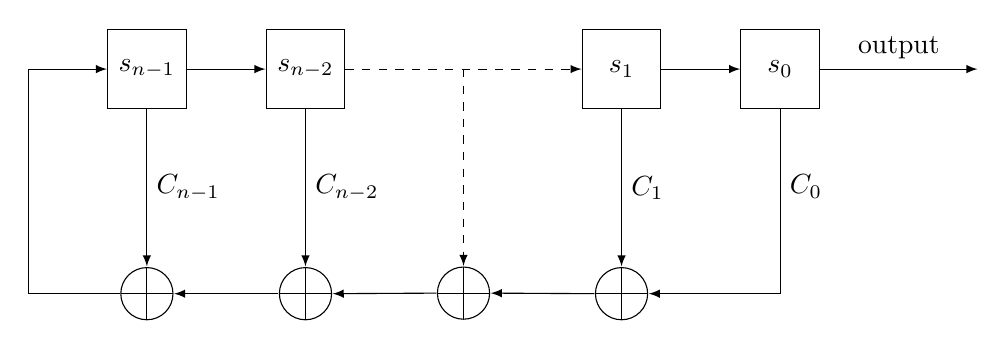
\begin{tikzpicture}


		\node[block                  ] (last_register) {$s_{n-1}$};
		\node[block, right = 1cm of last_register] (second_last_register) {$s_{n-2}$};
		\draw[line] (last_register.east) -- (second_last_register.west) ;

		\node[block, right = 3cm of second_last_register] (second_register) {$s_{1}$};
		\node[block, right = 1cm of second_register] (mid_register) {$s_{0}$};
		\draw[line] (second_register.east) -- (mid_register.west) ;

		\draw[dashed, line] (second_last_register.east) -- (second_register.west) ;

		\node[coordinate, right = 2cm of mid_register] (output_point) {};
		\draw[line] (mid_register.east) -- (output_point.west) node [midway, above] {output};

		\node[XOR, scale=2, below = 2cm of second_register] (first_xor) {};
		\draw[line] (second_register.south) -- (first_xor.north) node [midway, right] {$C_1$};
		\draw[line] (mid_register.south) |- (first_xor.east) node [pos=0.21, right] {$C_0$};

		\node[coordinate, right = 1.5cm of second_last_register] (h) {};
		\node[XOR, scale=2, below = 2.5cm of h] (mid_xor) {};
		\draw[line] (first_xor.west) -- (mid_xor.east) ;
		\draw[dashed, line] (h.south) -- (mid_xor.north) ;

		\node[XOR, scale=2, below = 2cm of second_last_register] (second_last_xor) {};
		\node[XOR, scale=2, below = 2cm of last_register] (last_xor) {};

		\draw[line] (second_last_register.south) -- (second_last_xor.north) node [midway, right] {$C_{n-2}$};
		\draw[line] (mid_xor.west) -- (second_last_xor.east) ;
		
		\draw[line] (second_last_xor.west) -- (last_xor.east) ;
		\draw[line] (last_register.south) -- (last_xor.north) node [midway, right] {$C_{n-1}$};

		\node[coordinate, left = 1cm of last_register] (return_point) {};
		
		\draw[line] (last_xor.west) -| (return_point) -- (last_register.west) ;




	\end{tikzpicture}
	\caption{Linear feedback shifter register of length $n$, with XOR gates.}
	\label{fig:lfsr}
\end{figure}


For PN sequences, there exists no formula for the cross-correlation of two different PN sequences. 
Exhaustive analysis is required to find out which sequences or entire sets have the cross-correlation characteristics that are good enough for the user's application.

The size of the code set is limited.
For a LFSR with $n$ registers, the maximum number of possible codes $C$ is given by \autoref{eq:num-of-pn-codes} \cite{mutagi1996pseudo}, where $P_i$ are the prime factors of $2^n - 1$ and $\alpha_i$ is the power of $i$th prime factor.

\begin{equation}
	\label{eq:num-of-pn-codes}
	C = \frac{1}{n} \prod \{ P_{i} ^ {(\alpha_i - 1)} \times (P_i - 1) \}
\end{equation}

For example when using a LFSR of size $n = 6$, $2^n - 1 = 63$, which can be factored into $3^2 \times 7$.
Giving $P_1 = 3$, $P_2 = 7$, $\alpha_1 = 2$ and $\alpha_2 = 1$.
Thus, the maximum number of codes is: $C = \frac{1}{6} \times \{ 3^{2 - 1} \times (3 - 1) \} \times \{ 7^{1 - 1} \times (7 - 1) \} = 6$.
Another example: Say there are going to be 144 user, so 144 codes are needed. 
This means a code length of 4095 chips.
















\subsection{Gold Sequences}

Gold sequences are a type of PN sequence. 
They are created by using two LFS registers as shown in \autoref{fig:gold-lfsr}.
In this figure there are two vectors $s$ and $t$ and two polynomials $C$ and $D$.
For a sequence to be constructed in this way that is a Gold sequence, only preferred pairs of polynomials can be used \cite{kedia2012comparative}.
When we have the polynomials $p(x)$ and $q(x)$, which are a preferred pair and produces the PN sequences $d_1$ and $d_2$ respectively, the resulting set of Gold codes is defined as can be seen in \autoref{eq:gold-def}, where $T^n$ represent the cyclic shift of $n$ bits.

\begin{equation}
	\label{eq:gold-def}
	Gold(d_1, d_2) = \{ d_1, d_2, d_1 \oplus d_2, d_1 \oplus Td_2, d_1 \oplus T^2d_2, \dotsc, d_1 \oplus T^{L - 1}d_2 \}
\end{equation}


\begin{figure}[h]
	\centering
	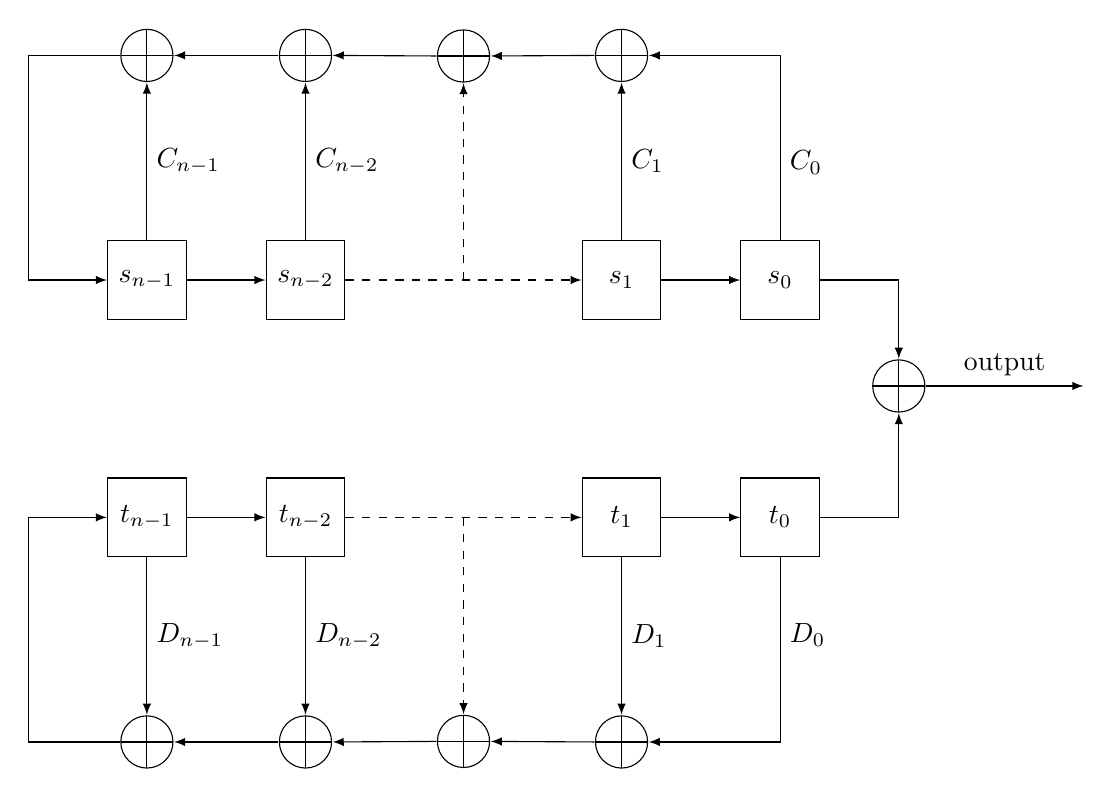
\begin{tikzpicture}

		\node[block                  ] (last_register1) {$s_{n-1}$};
		\node[block, right = 1cm of last_register1] (second_last_register1) {$s_{n-2}$};
		\draw[line] (last_register1.east) -- (second_last_register1.west) ;

		\node[block, right = 3cm of second_last_register1] (second_register1) {$s_{1}$};
		\node[block, right = 1cm of second_register1] (mid_register1) {$s_{0}$};
		\draw[line] (second_register1.east) -- (mid_register1.west) ;

		\draw[dashed, line] (second_last_register1.east) -- (second_register1.west) ;

		\node[coordinate, right = 1cm of mid_register1] (output_point1) {};

		\node[XOR, scale=2, above = 2cm of second_register1] (first_xor1) {};
		\draw[line] (second_register1.north) -- (first_xor1.south) node [midway, right] {$C_1$};
		\draw[line] (mid_register1.north) |- (first_xor1.east) node [pos=0.21, right] {$C_0$};

		\node[coordinate, right = 1.5cm of second_last_register1] (h1) {};
		\node[XOR, scale=2, above = 2.5cm of h1] (mid_xor1) {};
		\draw[line] (first_xor1.west) -- (mid_xor1.east) ;
		\draw[dashed, line] (h1.north) -- (mid_xor1.south) ;

		\node[XOR, scale=2, above = 2cm of second_last_register1] (second_last_xor1) {};
		\node[XOR, scale=2, above = 2cm of last_register1] (last_xor1) {};

		\draw[line] (second_last_register1.north) -- (second_last_xor1.south) node [midway, right] {$C_{n-2}$};
		\draw[line] (mid_xor1.west) -- (second_last_xor1.east) ;
		
		\draw[line] (second_last_xor1.west) -- (last_xor1.east) ;
		\draw[line] (last_register1.north) -- (last_xor1.south) node [midway, right] {$C_{n-1}$};

		\node[coordinate, left = 1cm of last_register1] (return_point1) {};
		
		\draw[line] (last_xor1.west) -| (return_point1) -- (last_register1.west) ;

		%%%%%%%%%%%%%%%%%%%%%%%%%%%%%%%%%%%%%%%%%%%%%%%%%%%%%%%%%%%%%%%%%%%%%%%%%%%%


		\node[block, below = 2cm of last_register1] (last_register) {$t_{n-1}$};
		\node[block, right = 1cm of last_register] (second_last_register) {$t_{n-2}$};
		\draw[line] (last_register.east) -- (second_last_register.west) ;

		\node[block, right = 3cm of second_last_register] (second_register) {$t_{1}$};
		\node[block, right = 1cm of second_register] (mid_register) {$t_{0}$};
		\draw[line] (second_register.east) -- (mid_register.west) ;

		\draw[dashed, line] (second_last_register.east) -- (second_register.west) ;

		\node[coordinate, right = 1cm of mid_register] (output_point) {};

		\node[XOR, scale=2, below = 2cm of second_register] (first_xor) {};
		\draw[line] (second_register.south) -- (first_xor.north) node [midway, right] {$D_1$};
		\draw[line] (mid_register.south) |- (first_xor.east) node [pos=0.21, right] {$D_0$};

		\node[coordinate, right = 1.5cm of second_last_register] (h) {};
		\node[XOR, scale=2, below = 2.5cm of h] (mid_xor) {};
		\draw[line] (first_xor.west) -- (mid_xor.east) ;
		\draw[dashed, line] (h.south) -- (mid_xor.north) ;

		\node[XOR, scale=2, below = 2cm of second_last_register] (second_last_xor) {};
		\node[XOR, scale=2, below = 2cm of last_register] (last_xor) {};

		\draw[line] (second_last_register.south) -- (second_last_xor.north) node [midway, right] {$D_{n-2}$};
		\draw[line] (mid_xor.west) -- (second_last_xor.east) ;
		
		\draw[line] (second_last_xor.west) -- (last_xor.east) ;
		\draw[line] (last_register.south) -- (last_xor.north) node [midway, right] {$D_{n-1}$};

		\node[coordinate, left = 1cm of last_register] (return_point) {};
		
		\draw[line] (last_xor.west) -| (return_point) -- (last_register.west) ;

		%%%%%%%%%%%%%%%%%%%%%%%%%%%%%%%%%%%%%%%%%%%%%%%%%%%%%%%%%%%%%%%%

		\node[XOR, scale=2, below = 1cm of output_point1] (gold_xor) {};
		\draw[line] (mid_register1) -| (gold_xor) ;
		\draw[line] (mid_register) -| (gold_xor) ;
		\node[coordinate, right = 2cm of gold_xor] (gold_output) {} ;
		\draw[line] (gold_xor.east) -- (gold_output.west) node [midway, above] {output};


	\end{tikzpicture}
	\caption{Two linear feedback shifter registers of length $n$, with XOR gates to produce a set of Gold sequences.}
	\label{fig:gold-lfsr}
\end{figure}

\begin{figure}
	\centering
	\includegraphics[width=\textwidth]{chapters/cdma-chapters/autocorr-gold.eps}
	\caption{Autocorrelation of one Gold sequence of length 1023.}
	\label{fig:autocorr-gold}
\end{figure}


\begin{figure}
	\centering
	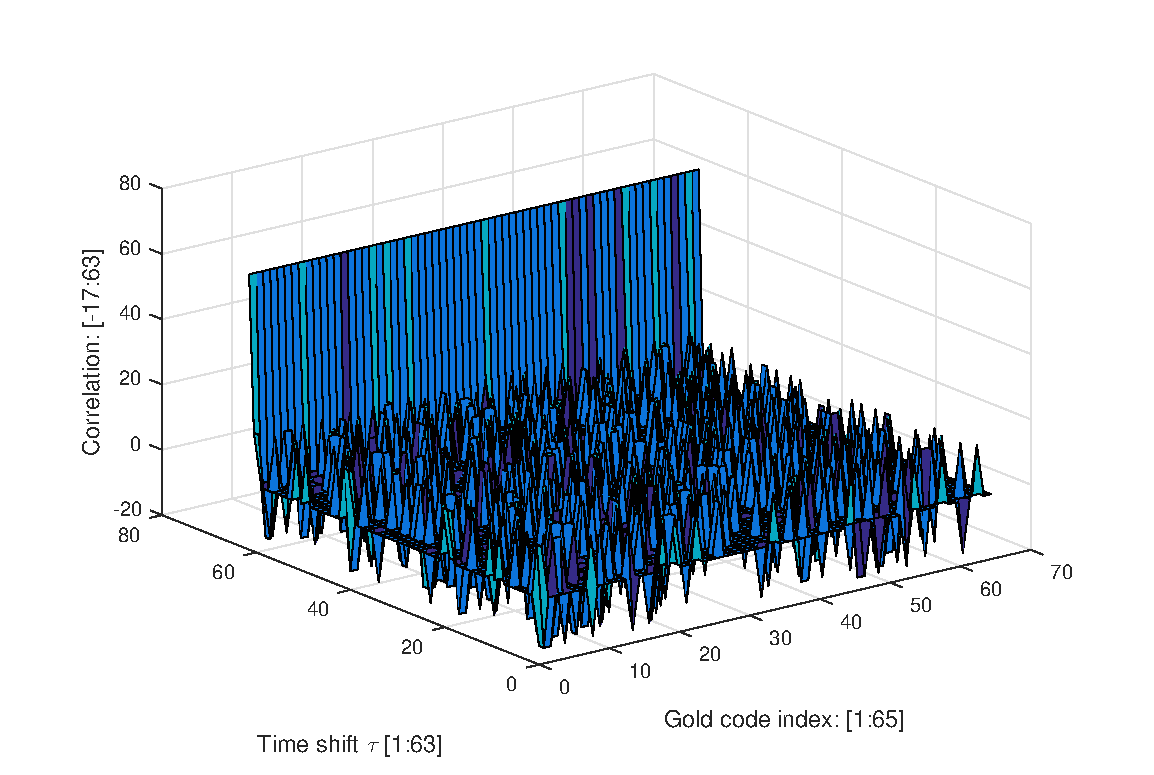
\includegraphics[width=\textwidth]{chapters/cdma-chapters/autocorr-gold-3d.eps}
	\caption{Autocorrelation of all Gold codes in the same set of length 63.}
	\label{fig:autocorr-gold-3d}
\end{figure}




The autocorrelation properties of Gold sequences are not as good as that of the PN sequences, as can be seen from \autoref{fig:autocorr-gold-3d}.
Apart from the original two PN sequences the autocorrelation values are not two-valued, but are four-valued.
See \autoref{eq:autocorr-gold} and \autoref{eq:gold-t(n)} for the autocorrelation properties of Gold sequences.

\begin{equation}
	\label{eq:autocorr-gold}
	R(\tau) = 
		\begin{cases}
			L    							& \quad \text{if } \tau = 0 \\
			\{ -t(n), \ -1, \ t(n) - 2  \} 	& \quad \text{if } \tau \neq 0 \\
		\end{cases}
\end{equation}

\begin{equation}
	\label{eq:gold-t(n)}
	t(n) = 
		\begin{cases}
			1 + 2^{\frac{n+1}{2}} & \quad \text{for odd } n \\
			1 + 2^{\frac{n+2}{2}} & \quad \text{for even } n \\
		\end{cases}
\end{equation}

See \autoref{eq:corsscorr-gold} and \autoref{eq:gold-t(n)} for the cross-correlation properties of Gold sequences \cite{mitra2008pseudo}.

\begin{equation}
	\label{eq:corsscorr-gold}
	R_{xy}(\tau) = 	\{ -t(n), -1, t(n) - 2  \} 
\end{equation}


From these equations it is clear to see that the absolute maximum cross-correlation is bounded by $t(n)$.

When $n$ is chosen to be odd, something can be said about the approximate frequency of occurrence of the cross-correlation values, see \autoref{tbl:freq-occurence-gold-cross-correlation} \cite{holmes2007spread}.

\begin{table}[h]
	\centering
	\begin{tabular}{ | l | l | }

		\hline
		$R_{xy}(\tau)$ 	& Frequency of occurrence	\\ \hline

		$-1$			& 0.5					 	\\ \hline
		$-t(n)$			& 0.25						\\ \hline
		$t(n) - 2$		& 0.25						\\ \hline

		

	\end{tabular}
	\caption{Table containing the approximate frequency of occurrence for all the cross-correlation values for $n$ odd.}
	\label{tbl:freq-occurence-gold-cross-correlation}
\end{table}

The Gold sequences posses good auto- and crosscorelation, suitable for a-synchronous usage.
\todo{Also state that this is extra good, because the LEDs/transmitters cannot be synchronized ???}
Also the codes scale well.
With a LFSR of $n$, the sequence length is $L = 2^n - 1$ and the number of sequences is $C = 2^n + 1$.

\todo{What information is really needed and which (like this table) is not necessary}












% !TeX root = ../../thesis.tex

\section{Mapping Problem}
\label{sec:mapping-problem}

The coding methods as discussed in \autoref{sec:orthogonal-sequences} and \autoref{sec:pn-sequences} are used in the field of telecommunication.
Since these signals are analog radio waves, the symbols are $+1$ and $-1$.
The orthogonal sequences generated via the Hadamard matrix can already be in this form, but the PN sequences contain only zeros and ones.
For the use with radio-signals the PN sequence is mapped to a form with $+1$ and $-1$, where the original $0$ is mapped to $+1$ and the original $1$ is mapped to $-1$.




The following proof \todo{Are we calling this a proof ??} shows how to calculate the correlation when the coding sequence consists of $+1$ and $-1$ symbols: 

\begin{proof}
	Let $s(t)$ be the received signal which is the composed signal of $m$ distinct codes.\\
	And let $c_i(t)$ be the code sequence $i$, and let $c_1(t)$ be the code for which we want to check if there is information there. \\

	\begin{align*}
		R(\tau)_{xy} = \displaystyle\sum_{t = 0} ^ {L - 1} x(t) \times y(t + \tau)	\tag{See \autoref{eq:correlation}}
		\\ \tau = 0,\ x = s(t),\ y = c_1(t)	
		\\ R(0)_{sc_{1}} = \displaystyle\sum_{t = 0} ^ {L - 1} s(t) \times c_1(t)
		\\ s(t) = \displaystyle\sum_{i = 1} ^ {m} c_i(t)														
		\\ R(0)_{sc_{1}} = \displaystyle\sum_{t = 0} ^ {L - 1}  \Bigg\{  c_1(t)	\times \displaystyle\sum_{i = 1} ^ {m} c_i(t) \Bigg\}
		\\ R(0)_{sc_{1}} = \displaystyle\sum_{t = 0} ^ {L - 1} \Bigg\{ c_1(t) \times c_1(t) + c_1(t) \times  \displaystyle\sum_{i = 2} ^ {m} c_i(t) \Bigg\} 
		\\ R(0)_{sc_{1}} = \displaystyle\sum_{t = 0} ^ {L - 1} c_1(t) \times c_1(t) + \displaystyle\sum_{t = 0} ^ {L - 1} \Bigg\{ c_1(t) \times  \displaystyle\sum_{i = 2} ^ {m} c_i(t) \Bigg\} 
		\\ R(0)_{sc_{1}} = L + \displaystyle\sum_{t = 0} ^ {L - 1} \Bigg\{ c_1(t) \times  \displaystyle\sum_{i = 2} ^ {m} c_i(t) \Bigg\} 
	\end{align*}

\end{proof}

So the result is $L$ plus the sum of all the other correlations. 
If the orthogonal sequences were used all the other correlations are zero.
If the Gold sequences were used each of the other correlations could be one of the values stated in \autoref{eq:corsscorr-gold}.
This is where the multiple access interference shows.



The above correlation calculation only holds up, when using a coding sequence which has the $+1$ and $-1$ symbols.
But when having LEDs which are modulating according to a sequence, the current draw is either on or off, a zero or a one.
This means a different correlation calculation is required.
First a formula for the mapping from $+1$ to zero and $-1$ to one is needed.
The formula can be found in \autoref{eq:radio-to-bin}, where $r$ denotes the $+1$ or $-1$ symbols and the outcome $b$ will be our binary value, i.e. $0$ or $1$.

\begin{equation}
	b = \frac{1 - r}{2}
	\label{eq:radio-to-bin}
\end{equation}


The previous proof can now be altered to incorporate the fact that the LEDs work with a one and zero state.


\begin{proof}
	Let $s(t)$ be the received signal which is the composed signal of $m$ distinct codes, which have symbols consisting of zero and one, which will be denoted be $c^b_i(t)$\\
	And let $c^r_i(t)$ be the code sequence $i$, and let $c^r_1(t)$ be the code for which we want to check if there is information there. \\
	Where $c^r_i(t)$ denotes a code sequence consisting of symbols $-1$ and $+1$.

	\begin{align*}
	T(\tau)_{xy} = \displaystyle\sum_{t = 0} ^ {L - 1} x(t) \times y(t + \tau)	\tag{See \autoref{eq:correlation}}
	\\ \tau = 0,\ x = s(t),\ y = c^r_1(t)
	\\ T(0)_{sc^r_{1}} = \displaystyle\sum_{t = 0} ^ {L - 1} s(t) \times c^r_1(t)	
	\\ s(t) = \displaystyle\sum_{i = 1} ^ {m} c^b_i(t)
	\\ T(0)_{sc^r_{1}} = \displaystyle\sum_{t = 0} ^ {L - 1} \Bigg\{  c^r_1(t)	\times \displaystyle\sum_{i = 1} ^ {m} c^b_i(t) 	\Bigg\}
	\\ T(0)_{sc^r_{1}} = \displaystyle\sum_{t = 0} ^ {L - 1} \Bigg\{  c^r_1(t)	\times \displaystyle\sum_{i = 1} ^ {m} \frac{1 - c^r_i(t)}{2}  	\Bigg\}
	\\ T(0)_{sc^r_{1}} = \frac{m}{2} \times \displaystyle\sum_{t = 0} ^ {L - 1} c^r_1(t) - \frac{1}{2} \times \displaystyle\sum_{t = 0} ^ {L - 1}  \Bigg\{ c^r_1(t) \times \displaystyle\sum_{i = 1} ^ {m} c^r_i(t) \Bigg\}
	\end{align*}

\end{proof}

This correlation calculation, denoted by $T$ now shows a different result than the previous result $R$.
Where $R = \displaystyle\sum_{t = 0} ^ {L - 1}  \Bigg\{  c_1(t)	\times \displaystyle\sum_{i = 1} ^ {m} c_i(t) \Bigg\}$ and $T = \frac{m}{2} \times \displaystyle\sum_{t = 0} ^ {L - 1} c^r_1(t) - \frac{1}{2} \times \displaystyle\sum_{t = 0} ^ {L - 1}  \Bigg\{ c^r_1(t) \times \displaystyle\sum_{i = 1} ^ {m} c^r_i(t) \Bigg\}$.
We can write it such that $R$ will become a function of $T$: 

\begin{proof}

	\begin{align*}
	T = \frac{m}{2} \times \displaystyle\sum_{t = 0} ^ {L - 1} c^r_1(t) - \frac{1}{2} \times R
	\\ R = m \times \displaystyle\sum_{t = 0} ^ {L - 1} c^r_1(t) - 2 \times T
	\end{align*}

\end{proof}

The sum of the sequence depends on the sequence used, when using orthogonal codes the sum will be zero, see \autoref{sec:orthogonal-sequences}.
If the sum is equal to zero, the factor $m$ will not matter.
However when the sequence used is a PN sequence or a balanced Gold sequence, the sum will be $-1$, This means: $R = -m - 2 \times T$, and then $m$, the number of signals, is important.
When using an unbalanced Gold sequence, the sum if that sequence can be calculated on the spot.











% CHAPTERS ... For instance: History/Prior Work, Design/Implementation, Experiments
%\include{chapters/chapter-2}

% CONCLUSIONS AND FUTURE WORK
% !TeX root = ../thesis.tex

\chapter{Conclusions and Future Work}
\label{chp:conclusionsandfuturework}

	\section{Conclusions}


	The aim of this thesis is to find out if lights could be identified as being on or off, by measuring the aggregated energy draw of those lights, with the help of VLC and a single smart-meter.
	CDMA codes have been investigated and compared to see which is the best suited for this scenario.
	Two solutions have been discussed to overcome the interference problem that comes with these types of codes.
	When these codes were understood and made usable in software simulations, two practical testbed were developed, for DC and AC, in order to experiment with.
	When the correct codes are used dependent on the size of the system, each individual light in each testbed could be successfully identified as being on or off in a timely manner.
	For larger systems a simulation was performed which shows that there can be made a trade-off between time and accuracy. 
	But the simulation showed that even with a high accuracy, the lights could still be identified in a timely manner.
	%As the testbed only represents a case where only these lights were connected, there is more work to be done when for instance there are also other appliances connected.






\section{Future Work}


This work is only the first step to disaggregate which lights are on and off.
There remains more work to be done, below there are ideas for future work.

	\subsection{Power Limiting Capacitor}

	The solution of using a capacitor in order to limit the power dissipated in the current source, introduced in \autoref{subsec:ac-modulator} can be further investigated.
	In particular what the drawbacks or benefits are of the of the current that is phase-shifted.
	And if the triggering circuit will still function properly or what the modifications are that need to be made in order for this scheme to work properly.


	\subsection{Other Appliances}

	As the testbeds represent cases where only these lights were connected, the question rises: What will happen when other appliances are connected ?
	These could for example be an incandescent light bulb or a refrigerator.
	To answer that question sample data from \cite{kolter2011redd} could be taken to represent some household appliances and added with the data of the modulation shown from the testbeds.
	Then signal filtering techniques could be performed to try and filter the signal from the modulating lights, given the fact that we know that these lights operate at a certain constant frequency.


	\subsection{Dimming Lights}

	LEDs can be often too bright for a persons liking, so the lights are dimmed.
	Dimming of an LED can be done in two ways: PWM, by lowering the duty cycle and so less power is dissipated by the LED or by limiting the current that flows through the LED.
	Since the LEDs are modulating via an OOK scheme, PWM cannot be used so instead current limiting must be done in order to dim the lights.
	But the CDMA codes are designed to work with each transmitter or LED has the same amplitude or in this case the same current.
	By dimming the LED and changing the current the codes may not work anymore.
	A solution for this can be that each LED will have multiple dimming levels and that for each dimming level other frequencies are used to modulate at.
	A filter can then be used to filter between these LEDs which all have the same amplitude.



	\subsection{Transmitting Data}

	With the current state of this system the LEDs can be identified as being on or off by detecting if their unique code is present or not.
	This can be seen as transmitting data, namely one bit, if the LED is on or off.
	If the LED needs to send other data about the status of the light two approaches can be thought of: 


	\begin{itemize}
		\item The unmodified code assigned to the light will be transmitted for the data-bit `0' and the negation of the code will be transmitted for the data-bit `1'. 
		This gives a problem with the definition of the cross-correlation, which is defined only for the unmodified codes. 
		When the negation of the codes is also used, the cross-correlation between the LEDs that are transmitting is no longer bounded by the mathematical formula and all the calculation on how many LEDs can transmit at the same time can no longer be used with these codes.
		It can be investigated if other codes do have a cross-correlation definition where the negation of the codes is also taken into consideration.

		\item Assign two unique codes from the same set to each light. 
		The lights will send the first code for the data-bit `0' and the second code for the data-bit `1'.
		Since the cross-correlation is defined for the codes from the same set this solution should not yield any problems.
		But further investigation may be required to see if this is a viable solution.
	\end{itemize}


	














% BIBLIOGRAPHY
%#define SORTED 1
\bibliographystyle{bib/latex8}
\bibliography{bib/mycollection}

%\appendix

%\include{appendix_a}

\end{document}

